

\documentclass[a4paper,onecolumn]{report}
\usepackage{caption}
\usepackage{subcaption}
\usepackage{setspace}
\usepackage{amssymb}
\usepackage[fleqn]{amsmath}
\usepackage{cite}
\usepackage{graphicx}
\usepackage{color}
\usepackage{float}
\usepackage[toc,page]{appendix}
\usepackage[nottoc]{tocbibind}
\usepackage{titlesec}
\usepackage{float}
\usepackage{setspace}
\titleformat{\chapter}{\normalfont\huge}{\thechapter.}{15pt}{\huge}
\renewcommand*{\familydefault}{\sfdefault}
\hyphenpenalty=5000 
\tolerance=1000

\usepackage[a4paper]{geometry}
\voffset=-80pt
\hoffset=0pt
\topmargin = 0pt
\textwidth = 450pt
\textheight = 770pt
\marginparwidth = 10pt
\oddsidemargin = 5pt
\topmargin = 1pt
\graphicspath{ {/images/} }

\setcounter{tocdepth}{2}

\begin{document}

%----------------------------------------------------------------------------------------
%	TITLE SECTION
%----------------------------------------------------------------------------------------

\begin{titlepage}

\newcommand{\HRule}{\rule{\linewidth}{0.5mm}}
\newcommand{\horrule}[1]{\rule{\linewidth}{#1}}

\center % Center everything on the page

\textsc{\small DELFT UNIVERSITY of TECHNOLOGY}\\[2.5cm] % Name of your university/college

\textsc{\LARGE Artificial Neural Networks}\\[0.5cm] % Major heading such as course name

\HRule \\[0.1cm]
\begin{spacing}{1.6}
{ \huge PROJECT PROPOSAL UPDATE}\\[-0.4cm] % Title of your document
\end{spacing}
\HRule \\[1.5cm]

\begin{minipage}{0.4\textwidth}
\begin{flushleft} \large
\emph{Authors:}\\
Michiel \textsc{Bongaerts\\}
Marjolein \textsc{Nanninga}\\
Tung \textsc{Phan}\\
Maniek \textsc{Santokhi}
\end{flushleft}
\end{minipage}
~
\begin{minipage}{0.4\textwidth}
\begin{flushright} \large
\end{flushright}
\end{minipage}\\[4cm]

{\large \today}\\[3cm]


\vfill

\end{titlepage}

%----------------------------------------------------------------------------------------
%	CONTENT
%----------------------------------------------------------------------------------------

\tableofcontents

\chapter{Introduction}

Mapping the world around us has always been a human endeavour to advance economical output. A better understanding of the places around us makes for more efficient travelling and exploitation of the land. However, it has always been a very slow and tedious process to produce these maps, something technology has not changed just yet.
\\
A new opportunity has arisen with the arrival of satellite imagery and an ever increasing amount of computational power. An opportunity where this mapping can be done automatically so that this tedious and slow job can be processed even more quickly and perhaps more accurately. It is with this in mind we further analyse any possibilities.\\
\\
This paper proposes an update. Now a more straightforward approach has been chosen in which the emphasis lies on the actual neural network rather than the conversion of interpreted images to vector graphic maps. The new approach deals with image patches rather than pixels. This document discusses the newly acquired concept with a list of features and the actual implementation details. Also an updated schedule will be presented. 

\chapter{Concept}

\section{Impression}
\begin{figure}[ht!]
    \centering
    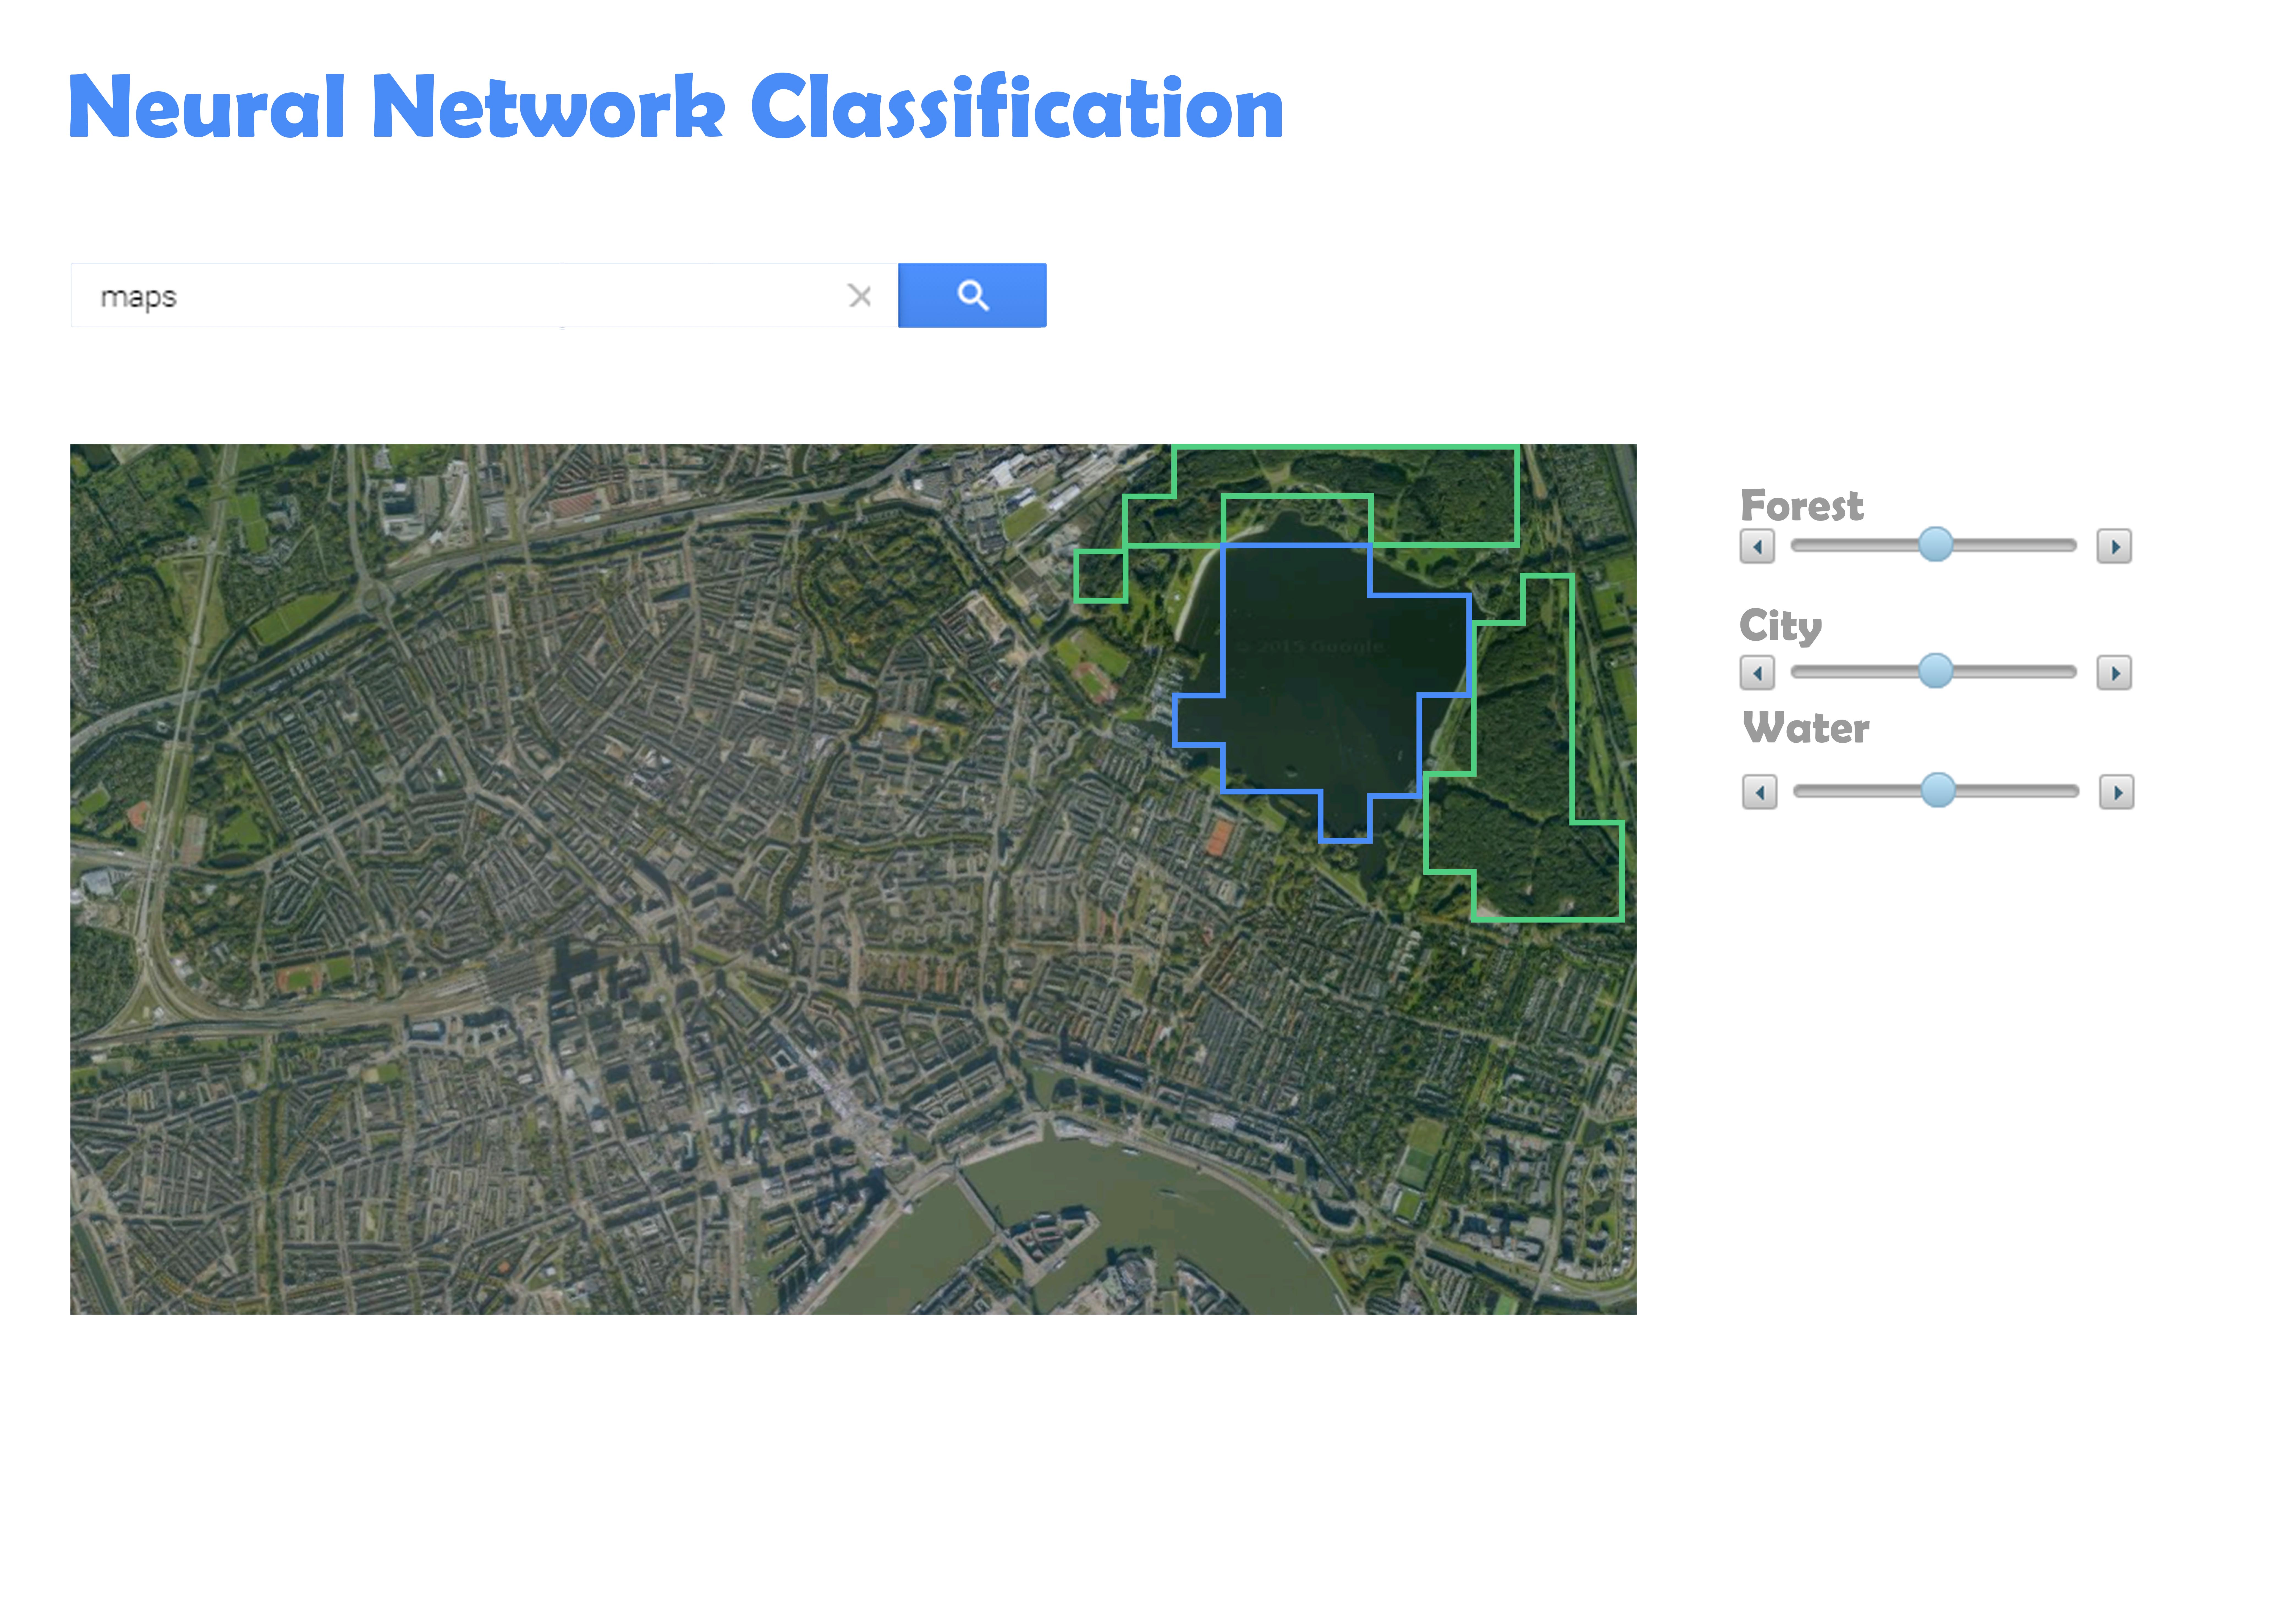
\includegraphics[width=1\textwidth]{interface.jpg}
    \caption{Impression of what the user interacts with.}
\end{figure}

\section{MoSCoW}
% Categories

\chapter{Implementation}

\section{Dataset}

\section{CNN}

\chapter{Schedule}

\end{document}



